\documentclass[9pt, aspectratio=169]{beamer}

\usetheme{metropolis}
\setbeamertemplate{itemize items}{\faAngleRight}

\metroset{titleformat=smallcaps,block=fill,numbering=counter,progressbar=frametitle,sectionpage=none}
\setbeamersize{text margin left=5mm,text margin right=5mm} 
% \input{embed_video}
\usepackage{fontspec,minted}
\usepackage[scale=1]{ccicons}
\usepackage{metalogo}
\usepackage{xcolor,colortbl}
\usepackage{multicol,multirow,booktabs}
\usepackage{appendixnumberbeamer}
\usepackage{graphicx}
\usepackage{mismath}
\usepackage{bm}
\usepackage{fontawesome5}
\usepackage{csquotes}
%\usepackage[backend=biber, natbib, sorting=nyt, doi=true, url=false, url=false, isbn=false, maxbibnames=10]{biblatex}
%\addbibresource{../../utils/refs.bib}

\usepackage[spanish, es-nodecimaldot]{babel}
\deftranslation[to=spanish]{Definition}{Definición}
\deftranslation[to=spanish]{Theorem}{Teorema}
\deftranslation[to=spanish]{Example}{Ejemplo}

\usepackage{mathtools, mathrsfs}
\usefonttheme{professionalfonts}
\usepackage{textcomp, wasysym}

\setsansfont[BoldFont={Iwona Bold}, Numbers={Lining, Proportional}]{Iwona Light}
% \setmathsfont(Digits)[Numbers={Lining, Proportional}]{Fira Sans Light}
\setmonofont[Scale=MatchLowercase]{DejaVu Sans Mono}

\setbeamercolor{alerted text}{fg=red,bg=black!2}
\setbeamercolor{progress bar}{fg=red,bg=red!2}
\setbeamertemplate{itemize item}{\faCaretRight}
\setbeamertemplate{itemize subitem}{ \faAngleRight}
\setbeamertemplate{blocks}[shadow=false]
\setbeamercolor{block title}{bg=black!30,fg=red}
\setbeamercolor{block body}{bg=black!20,fg=black}
\setbeamertemplate{theorem begin}
{%
\begin{\inserttheoremblockenv}
{%
\inserttheoremheadfont
%{Teorema:}
\inserttheoremname
\ifx\inserttheoremaddition\@empty\else\ : \inserttheoremaddition\fi%
\inserttheorempunctuation
}%
}
\setbeamertemplate{theorem end}{\end{\inserttheoremblockenv}}
\makeatother


 
\usepackage{gensymb,amssymb}
\usepackage{upquote}
\usepackage{cancel}
\usepackage{algpseudocode}
\algrenewcommand\algorithmicrequire{\textbf{Requiere}}
\algrenewcommand\algorithmicensure{\textbf{Devuelve}}
\setbeamertemplate{blocks}[shadow=false]

\newcommand{\cx}{\column{0.5\textwidth}}
\newcommand{\cw}[1]{\column{#1\textwidth}}

\author{Manuel Carlevaro}
\date{}
\institute{
  \vspace{6em}
  \centering
  {\tiny
  Universidad de Navarra \enspace • \enspace 2024 
} }

%% Operadores
\DeclareMathOperator{\sen}{sen}
\DeclareMathOperator{\senc}{senc}
\DeclareMathOperator{\sign}{sign}
\newcommand{\T}[1]{\underline{\bm{#1}}}
\DeclareMathOperator{\Tr}{Tr}
\DeclareMathOperator{\rg}{rg}
\DeclareMathOperator{\cond}{cond}

\usepackage{hyperref}
\hypersetup{
    colorlinks,
    citecolor=blue,
    filecolor=black,
    linkcolor=blue,
    urlcolor=blue
}
\urlstyle{same}


\usepackage{tikz}
\usetikzlibrary{shapes,shadows,arrows,positioning,matrix,chains,backgrounds,fit}

\tikzset{
    %Define standard arrow tip
    >=stealth',
    %Define style for boxes
    obj/.style={
           rectangle,
           rounded corners,
           draw, very thick,
           text width=10em, fill=green!20,
           minimum height=2em,
           text centered, drop shadow},
    proc/.style={
	    rectangle, rounded corners,
	    draw,fill=red!50,very thick,
	    text width=8em,minimum height=2em,
	    text centered, drop shadow},
    % Define arrow style
    pil/.style={
           ->,
           thick,
           shorten <=2pt,
           shorten >=2pt,}
}

%\setbeamertemplate{bibliography item}{%
  %\ifboolexpr{ test {\ifentrytype{book}} or test {\ifentrytype{mvbook}}
    %or test {\ifentrytype{collection}} or test {\ifentrytype{mvcollection}}
    %or test {\ifentrytype{reference}} or test {\ifentrytype{mvreference}} }
    %{\setbeamertemplate{bibliography item}{\faBook}}
    %{\ifentrytype{online}
            %{\setbeamertemplate{bibliography item}{\faGlobe}}
   %{\setbeamertemplate{bibliography item}{\faFileText}}}%
  %\usebeamertemplate{bibliography item}}

%\defbibenvironment{bibliography}
  %{\list{}
     %{\settowidth{\labelwidth}{\usebeamertemplate{bibliography item}}%
      %\setlength{\leftmargin}{\labelwidth}%
      %\setlength{\labelsep}{\biblabelsep}%
      %\addtolength{\leftmargin}{\labelsep}%
      %\setlength{\itemsep}{\bibitemsep}%
      %\setlength{\parsep}{\bibparsep}}}
  %{\endlist}
  %{\item}
%\newcommand{\bcite}[1]{\citeauthor{#1}, \citetitle{#1} (\citeyear{#1})}


\title{Introducción a la física}
\subtitle{Magnitudes y sistemas de unidades. Análisis dimensional. Proceso de medida y teoría de errores.}


\begin{document}
\maketitle

\begin{frame}{ Objetivos }

\begin{itemize}
 \item Recordar el concepto de medición y unidad de medida.
 \item Repasar las diferentes magnitudes básicas, sus unidades, múltiplos y submúltiplos.
 \item Repasar las reglas para conversión de unidades.
 \item Aprender a representar la incertidumbre de una medida.
\end{itemize}

\end{frame}

\begin{frame}
  \frametitle{Magnitudes físicas}
  \begin{definition}[Magnitud o cantidad física]
    Una \textbf{magnitud} o \textbf{cantidad física} es una propiedad de un sistema físico que puede ser \textbf{cuantificada} por medio de una {medición} o de una relación de medidas.

    Se expresa como un \textbf{valor}, que es una multiplicación de un \textbf{valor numérico} y una \textbf{unidad de medición}.
  \end{definition}
\pause

\begin{example}[Masa de un cuerpo]
    \[ M = \underbracket[.25pt]{94.5}_{\text{valor numérico}} \times \overbracket[.52pt]{\text{kg}}^{\text{unidad de medición}} = \qty{94.5}{kg} \] 
\end{example}

\begin{columns}[t]
\cx
\textbf{Magnitudes básicas:}
\begin{itemize}
 \item Longitud (altura, distancia, profundidad, diámetro, perímetro, ...)
 \item Masa (inercia)
 \item Tiempo (duración, retraso, ...)
\end{itemize}
\cx
\textbf{Magnitudes derivadas:}
\begin{itemize}
    \item Velocidad, aceleración
    \item Area, volumen
    \item Fuerza
\end{itemize}
\end{columns}

%\begin{alertblock}{\centering \faInfoCircle}
%Algunos autores las llaman indistintamente magnitudes o cantidades físicas.
%\end{alertblock}

\end{frame}


\begin{frame}{Medir es comparar}
\begin{example}[Mediciones]
\begin{itemize}
 \item La {\bf longitud} de la mesa mide igual que el diámetro de 8 platos. 
 \item El {\bf tiempo} para caminar de Pamplona a Madrid es igual a 3.1 veces el tiempo que la tierra tarda en dar una vuelta sobre su eje.
 \item La {\bf masa} de la manzana es 0.5 veces la de un vaso de leche.
\end{itemize}
\end{example}
\pause

\vspace{0.3cm}
{\bf Sistema Internacional (SI)}
\begin{columns}[c]
\cw{0.4}
\begin{center}
\includesvg[width=0.6\textwidth]{figs/SI.svg}

{\tiny Fuente: \href{https://es.wikipedia.org/wiki/Archivo:SI_Logo_with_defining_constants.png}{Wikimedia Commons}}
\end{center}

\cw{0.6}
\only<2> {
\textbf{Algunas unidades básicas:}
\begin{itemize}
    \item Tiempo [t] $\rightarrow$ {\bf segundo} (s): \num{9192631770} veces el período de la microonda necesaria para excitar los átomos de cesio.
    \item Longitud [l] $\rightarrow$ {\bf metro} (m): distancia que recorre la luz en el vacío en $1/$\num{299792458} segundos].
    \item Masa [m] $\rightarrow$ {\bf kilogramo} (kg): se fija la constante de Plank: $h=$ \qty{6.62607015e-34}{kg.m^2/s^{-1}}.
\end{itemize}
}
\only<3> {
\begin{example}[Mediciones SI]
\begin{itemize}
    \item La longitud de la mesa mide \qty{1.6}{m}. 
    \item El tiempo para caminar de Pamplona a Madrid es de \qty{273600}{s}.
    \item La masa de la manzana es de \qty{0.1}{kg}.
\end{itemize}
\end{example}
}
\end{columns}
\end{frame}

\begin{frame}{Prefijos}
\begin{center}
  \begin{tabular}{lccclcc}
    \toprule
    \textbf{Prefijo} &\textbf{Símbolo} & \textbf{Exponente} & & \textbf{Prefijo} & \textbf{Símbolo} & \textbf{Potencia} \\
    \midrule
      quecto & \unit{\quecto\nada} & \num{d-30} & & deca & \unit{\deca\nada} &   1 \\
      ronto & \unit{\ronto\nada}  & \num{d-27} &  & hecto & \unit{\hecto\nada}  &  \num{d2} \\
      yocto & \unit{\yocto\nada}  & \num{d-24} &  & kilo & \unit{\kilo\nada}  &  \num{d3} \\
      zepto & \unit{\zepto\nada}  & \num{d-21} &  & mega & \unit{\mega\nada}  &  \num{d6} \\
      atto & \unit{\atto\nada}  & \num{d-18} &  & giga & \unit{\giga\nada}  &  \num{d9} \\
      femto & \unit{\femto\nada}  & \num{d-15} &  & tera & \unit{\tera\nada}  &  \num{d12} \\
      pico & \unit{\pico\nada}  & \num{d-12} &  & peta & \unit{\peta\nada}  &  \num{d15} \\
      nano & \unit{\nano\nada}  & \num{d-9} &  & exa & \unit{\exa\nada}  &  \num{d18} \\
      micro & \unit{\micro\nada}  & \num{d-6} &  & zetta & \unit{\zetta\nada}  &  \num{d21} \\
      mili & \unit{\milli\nada}  & \num{d-3} &  & yotta & \unit{\yotta\nada}  &  \num{d24} \\
      centi & \unit{\centi\nada}  & \num{d-2} &  & ronna & \unit{\ronna\nada}  &  \num{d27} \\
      deci & \unit{\deci\nada}  & \num{d-1} &  & quetta & \unit{\quetta\nada}  &  \num{d30} \\
    \bottomrule
  \end{tabular}
\end{center}


\begin{alertblock}{\centering \faInfoCircle}
El gramo (g) no se considera una unidad fundamental de masa, pero se usa para definir los múltiplos y submúltiplos de masa.
\end{alertblock}
\end{frame}

\begin{frame}{Ejemplos de escalas}
    \begin{center}
        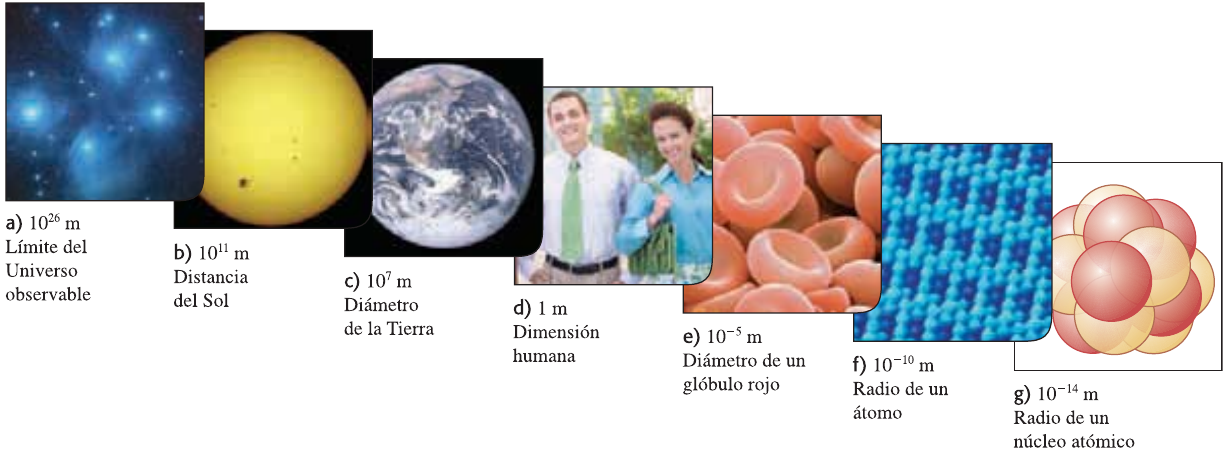
\includegraphics[width=0.9\textwidth]{figs/escalas-l.png}
    \end{center}
\begin{columns}[t]
\cx
\textbf{Masa:}
\begin{itemize}
    \item \qty{1}{\ug}: partícula pequeña de polvo
    \item \qty{1}{\mg}: grano de sal 
    \item \qty{1}{g}: sujetador de papeles
\end{itemize}

\cx
\textbf{Tiempo:}
\begin{itemize}
    \item \qty{1}{\ns}: tiempo en que la luz recorre \qty{0.3}{m}
    \item \qty{1}{\us}: tiempo en que la ISS recorre \qty{7.7}{mm}
    \item \qty{1}{\ms}: tiempo en que el sonido recorre \qty{0.35}{m}
\end{itemize}
\end{columns}
\end{frame}


\begin{frame}
  \frametitle{Expresión de cantidades físicas y consistencia de unidades}
\Large
\begin{itemize}
    \item Las unidades en que se mide una magnitud son más importantes que el número específico. Si el resultado correcto es \qty{3.5}{\cm} y por un error obtuve \qty{8.3}{\cm} es mucho mejor que si obtengo \qty{3.5}{\kg}, \qty{3.5}{\dm} o \num{3.5}.
 \item Una cantidad específica puede representarse con un símbolo algebraico (por ejemplo, una letra en itálica) ($a$, $h$, $x$, $t$, $\phi$, etc). Esta letra representa al número y la unidad juntos. Las unidades no van en itálica. 
 \item Las ecuaciones deben ser {\bf consistentes} en sus unidades. Sólo pueden sumarse, restarse o compararse cantidades con unidades iguales (metros con metros, etc).
 \item Si debo sumar, restar o comparar cantidades que están expresadas en diferentes múltiplos o submúltiplos de una misma unidad fundamental puedo hacer {\bf conversión} de unidades.
 \item Los símbolos de las unidades se operan en forma algebraica como una cantidad cualquiera.
\end{itemize}

\end{frame}


\begin{frame}
  \frametitle{Estrategias}
\Large
\begin{itemize}
    \item Convertir primero todas las unidades en SI (\unit{m}, \unit{kg}, \unit{s}, etc.).
 \item Hacer las operaciones.
 \item Convertir el resultado a las unidades deseadas.
 \item Para convertir unidades se puede multiplicar y dividir por la misma cantidad expresada en dos múltiplos (o submúltiplos) diferentes: $\frac{\qty{1}{m}}{\qty{1000}{mm}}$, $\frac{\qty{60}{s}}{\qty{1}{min}}$, $\frac{\qty{1}{kg}}{\qty{1000000}{\micro g}}$, ... 
 \item Verificar la consistencia de las unidades de un resultado.
\end{itemize}
\end{frame}

\begin{frame}{Ejemplos}
\begin{example}[Conversión de unidades de rapidez] 
La Estación Espacial Internacional (ISS) orbita la Tierra a una altura de aproximadamente \qty{420}{km} a una velocidad de \qty{27600}{km/h}. Expresar esa rapidez en \unit{m/s}.
\pause
\[ \qty{27600}{km/h} = \left(\num{27600} \times 10^3 \frac{\unit{m}}{\unit{h}}\right) \left(\frac{\qty{1}{h}}{\qty{3600}{s}}\right) = \qty{7666.666}{m/s} \] 
\end{example}
\pause
\begin{example}[Conversión de unidades de volumen]
El diamante tallado más grande del mundo es la Primera Estrella de África (montado en el cetro real británico y guardado en la Torre de Londres). Su volumen es de \num{1.84} pulgadas cúbicas. ¿Cuál será su volumen en centímetros cúbicos? (\num{1} pulgada $= \qty{2.54}{cm}$.)
\pause
\[ \qty{1.84}{in^3} = (\qty{1.84}{in^3}) \left(\frac{\qty{2.54}{cm}}{\qty{1}{in}}\right)^3 = (\num{1.84})(\num{2.54})^3 \frac{\unit{in^3} \unit{cm^3}}{\unit{in^3}} = \qty{30.2}{cm^2} \]
\end{example}
\end{frame}

\begin{frame}
  \frametitle{Incertidumbre}
\Large
\begin{itemize}
 \item Las cantidades físicas no se pueden medir con exactitud infinita. Hay {\bf incertidumbre} o {\bf error}.
 \item La incertidumbre se puede expresar como \qty[separate-uncertainty=true]{3.5 \pm 0.2}{m} o en forma más compacta \qty{3.5 \pm 0.2}{m}.
 \item También se puede usar el error porcentual como \qty{3.5}{m} $\pm$  \num{2.9}\%. 
 \item Si no hay un error indicado se entiende que la última cifra significativa representa el error: \qty{3.5}{m} significa \qty{3.5 \pm 0.1}{m}, \qty{3.50}{m} significa \qty{3.50 \pm 0.01}{m} y \qty{347}{kg} significa \qty{347 \pm 1}{kg}.    
 \item \qty{300}{m} significa ¿?
\end{itemize}
\end{frame}

\begin{frame}{Incertidumbre y notación científica}
\Large
\begin{itemize}
    \item Notación científica: \num{300} $=$ \num{3d2} y \num{0.03} $=$ \num{3d-2}.
    \item \qty{3.00e2}{m} significa \qty[separate-uncertainty=true]{300 \pm 1}{m} o \qty{300 \pm 1}{m}. 
    \item \qty{3.0e2}{m} significa \qty[separate-uncertainty=true]{300 \pm 10}{m} o \qty{300 \pm 10}{m}.
    \item \qty{3e2}{m} significa \qty[separate-uncertainty=true]{300 \pm 100}{m} o \qty{300 \pm 100}{m}.
    \item \qty{3.0e-2}{m} significa \qty[separate-uncertainty=true]{0.03 \pm 0.001}{m}.
    \item \qty{3e-2}{m} significa \qty[separate-uncertainty=true]{0.03 \pm 0.01}{m}.
\end{itemize}

\vspace{0.2cm}
{\bf Operaciones}
\begin{itemize}
 \item $\times$ y $\div$: la menor cantidad de cifras significativas.
 \item $+$ y $-$: la mayor incertidumbre.
\end{itemize}
\end{frame}

\begin{frame}{Incertidumbre en operaciones algebraicas}
\begin{center}
    \begin{tabular}{p{4cm}p{8cm}}
        \toprule
        \textbf{Operación matemática} & \textbf{Cifras significativas en el resultado} \\
        \midrule 
        Multiplicación o división & No más que el número que tiene menos cifras significativas \\
                                  & \textit{Ejemplo:} $\num{0.745} \times \num{2.2} / \num{3.885} = \num{0.42}$ (no \num{0.4218790219}) \\
                                  & \textit{Ejemplo:} $\num{1.32578e7} \times \num{4.11e-3} = \num{5.45e4}$ \\
        Suma o resta & Lo determina el número con mayor incertidumbre (es decir, el menor número de dígitos a la derecha del punto decimal) \\
                     & \textit{Ejemplo:} $\num{27.153} + \num{138.2} - \num{11.74} = \num{153.6}$ (no \num{153.613})\\
        \bottomrule
    \end{tabular}
\end{center}

\begin{alertblock}{\centering \faExclamationTriangle}
No dar un resultado con más cifras significativas que los datos con que fue calculado.
\end{alertblock}

\begin{center}
{\Large \faArrowCircleRight \faPen* Actividad 1}
\end{center}

\end{frame}


\end{document}

